 \section{Safety and Efficacy of Closed-loop Medical Devices}
\subsection{Motivation}
Medical devices play an essential role in the care of patients around the world, and can have a life-saving effect.
To cite one example, an estimated 3 million people worldwide have implanted pacemakers (a heart rhythm adjustment device), with \~600,000 added annually.
In the US, $\sim$800,000 people have an implanted defibrillator (a heart rhythm management device), with 10,000 added monthly.
Clinical trials have presented evidence that patients implanted with defibrillators have a mortality rate reduced by up to 31\%.
Financially, the medical device market is worth \$289 billion.
Examples include everything from adhesive bandages to drug infusion pumps, surgical robots, deep brain stimulation systems and devices still undergoing basic research like the artificial pancreas.
These are safety-critical technologies combining hardware and software, each of which must be rigorously validated to be efficacious and safe.

There are two categories of medical devices. 
One category is the \emph{open-loop medical device} which has either therapeutic or diagnostic capability but not both.
An example is infusion pumps that inject fluid into the patient's system.
Open-loop medical devices are normally operated by professional medical care providers, and this provides safety guarantees.
On the other hand, the fast-growing category of \emph{closed-loop medical devices} has both therapeutic and diagnostic capability, and often operate \emph{without} physician intervention.
In other words they are, by and large, autonomous.
An example is the implantable pacemaker: it diagnoses the patient's heart rhythm by sensing cardiac electrical activity via direct contact with the heart muscle.
Software embedded in the pacemaker then determines when to deliver electrical pacing to maintain appropriate rhythm (Fig. \ref{fig:pacemaker}). 
Closed-loop medical devices often interact with the human physiology without the physician's intervention.
%\mynote{HA}{the jump from 'without physician intervention' to 'serious injury' is not justified}
Therefore device failures like inappropriate therapies cannot be intervened in time, which may result in serious injuries or death of the patient.
As a result, closed-loop medical devices are categorized by regulation agencies like the US FDA as the highest risk devices.
\begin{figure}[t]
	\centering
	\includegraphics[scale=0.33]{figs/fig1pacemaker.pdf}
	\caption{\small Pacemaker operating in a closed-loop with the heart. The leads sense cardiac electrophysiological activity from inside the heart tissue (AS/VS = Atrial/Ventricular Sense event) and actuate the heart (AP/VP = Atrial/Ventricular Pacing event to maintain a desired heart rate.}
	\label{fig:pacemaker}
\end{figure}

\subsection{Challenges for Developing Safe Closed-loop Medical Devices}
\subsubsection{Complex Software}
To guarantee safe operation, closed-loop medical devices need to correctly identify the current medical condition of the patient and deliver an appropriate level of therapy when needed.
The complex run-time diagnoses needed for closed loop performance, and the intricate therapy delivered, have driven most diagnosis and therapy functions into software.
This software has grown in complexity: 
implanted cardiac pacemakers and defibrillators (ICDs), for example, have 80,000-100,000 lines of software code that essentially make all sensing and actuation decisions autonomously within the human body, over the 5-7 years device lifetime. 
According to the US Food and Drug Administration (FDA), in 1996, 10\% of all medical device recalls were caused by software-related issues. 
This percentage rose to an average of 15\% of recalls from 2008 to 2012. 
 
\subsubsection{Closed-loop Interaction with Human Physiology}
One driver of software complexity is the fact that it interacts with human physiology. 
Physiology is much more complex and less well-understood than man-made systems like cars and airplanes, and spans several scales from the molecular to the entire human body.
Cellular interactions give rise to emergent behavior at the organ and body levels.
Drugs taken by a patient can affect the efficacy and even the safety of the medical device.
Moreover, the variability between humans is orders of magnitude greater than that between two cars coming off the assembly line.
%Using the pacemaker as an example of closed-loop device, and the heart as the organ to be modeled, we present several of the challenges and early results in model-based verification.

\subsection{Evaluating the closed loop}
The safety and efficacy of a closed-loop medical device can only be measured when the device is connected to the organ or physiology it is affecting, i.e, when it is in the closed loop. 
E.g., the ICD must be observed when connected to a human heart.
Currently the only time this happens is during \emph{clinical trials}.
In a clinical trial, devices are implanted in a group of patients and their safety and efficacy are evaluated.
Clinical trials are costly in terms of time and money, and expose enrolled patients to unproven therapies.
Problems found at this late stage are also very costly to fix.

Thus, the primary challenge of designing high-confidence medical device software is to guarantee that the device will never drive the patient into an unsafe condition,
even though we do not have complete understanding of that patient's physiology, and the device has limited sensing capabilities from which to infer the patient's current condition. 

%We may classify devices as open-loop or closed-loop.
%A \emph{closed-loop device} like a pacemaker is in a feedback loop with the organ(s) it affects (see Fig.\ref{fig:pacemaker}): it monitors certain physiological variables like heart rate, and delivers therapy, in the form of low-energy electrical pulses, to maintain a healthy heart rate.
%Another example is the artificial pancreas, which monitors blood glucose levels and delivers therapy, in the form of insulin, to maintain safe glucose levels.
%An \emph{open-loop device} on the other hand, either, (a) like a drug infusion pump, does not measure any physiological variables: the therapy it delivers is pre-programmed and non-reactive; or (b) only measures physiological signals but does not deliver therapy, as in the case of a blood pressure monitor.
%Open-loop devices

%Closed-loop devices require very little physician intervention after the discharge visit, and hence permit a better lifestyle.
%Because they are constantly monitoring the physiological variables, they permit a more timely delivery of therapy. 
%The complex run-time diagnoses needed for closed loop performance, and the intricate therapy delivered, has driven most diagnosis and therapy functions into software.
%This software is life-critical and verification methods should provide a high confidence in its correctness.
%

\begin{figure}[t]
	\centering
	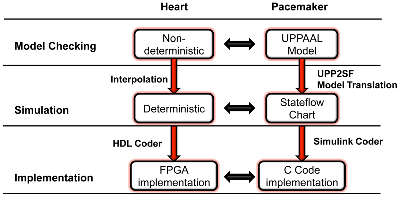
\includegraphics[scale=0.35]{figs/model_based_b.pdf}
	\caption{\small Model-based design of pacemaker software.}
	\label{fig:MBD}
\end{figure}
\subsection{Model-based Design}
\emph{Model-based Design (MBD)} enables a form of closed-loop validation at earlier design stages, which can potentially save development cost, and increase the chances of a successful clinical trial.
%\mynote{HA}{let's not use the word plant in this, it's too out of context.}
In MBD, the device (or a model thereof) is connected to a \emph{model} of the physiological system it interacts with.
%By high confidence verification, researchers mean that under all possible behaviors of the physiological models, the device will act correctly.
Using the pacemaker as an example of closed-loop device, and the heart as the organ to be modeled, we present several of the challenges and early results in model-based verification.

Fig. \ref{fig:MBD} demonstrates our model-based design framework for pacemaker software.
%Throughout the development process we developed heart models to interact with the pacemaker model in closed-loop. 
This framework can potentially be applied for developing other closed-loop medical devices.
There are several key steps within the framework:
\subsubsection{Risk Analysis with Model Checking}
%\mynote{HA}{first paragraph not clear - re-organize as follows: Risk analysis is this. It is mandated by FDA. In MBD, we used model checking to do risk analysis. MC is this. it is used in semiconductor industry. We used it for irsk analysis like this.}
Risk analysis is an activity identifies potential risks of the device and analyze how well they are mitigated.
Risk analysis is mandated by the regulators as a mean to evaluate the safety of the medical devices.
Model checking has been widely used in the semiconductor industry.
It can check the whole state space of a model for property violations.
%Risk analysis is an activities mandated by the regulator to ensure the safety of the device.
By specifying the risks as properties, and model checking the closed-loop model which consists of the device model and a physiological model, we can automate the risk analysis process and make it more rigorous.
With tools like quantitative model checker, we can also evaluate the frequency and severity of the remaining risks.
All of the analysis above can be used as evidence for the safety of the device model.

\mynote{HA}{this also needs re-writing...}
The major challenge for closed-loop model checking is to develop appropriate physiological models. 
The models should be general enough to cover physiological behaviors from multiple patient conditions, while at the same time expressive enough to maintain physiological meaning of an execution trace.
There is no single model that can satisfy both requirements and for different properties, different models are required.
It is therefore important to have a rigorous hierarchy of physiological models with different abstraction levels and a procedure to choose the appropriate model for a property.

\subsubsection{Validated Model to Validated Code}
In MBD, the code that runs inside a device is generated from the verified model.
It is essential that the generated code also satisfy the safety and efficacy properties of the model.
In our framework, we developed a model translation tool which rigorously translates a device model from the UPPAAL model checker to a Stateflow chart.
The Stateflow chart can then be compiled into C code implementation using Simulink Coder, which completes a tool chain from validated model to validated code.

Due to the limited semantics of most model checking tools, the device model in the model checker is generally an abstraction of the actual device functions.
The biggest challenge for translating a verified model to verified code is how to deal with the additional behaviors in the actual implementation, and how they affect the code's properties, like safety.

\subsubsection{Model-based Clinical Trials}
%Clinical trials for medical devices are costly in terms of both time and money, therefore they should be carefully planned to reduce the risk of failures.
Clinical trials for new high-risk devices are planned using data from previous trials and small-scale studies. 
Relying on historical data has the shortcoming that previously studied populations may not be comparable to the population of the current trial.
Moreover, the efficacy of the new device \emph{on a particular study population} can not be known before the trial is actually conducted, and yet must be estimated before trial start.
Thus some of the assumptions in the trial's study protocol may be invalid, causing the trial to fail to meet its desired objectives (e.g., showing superiority of the device over the current one).

We are proposing \emph{Model-based Clinical Trials (MBCT)}, which use computer models of the physiology to generate a virtual patient population and run trials on it to evaluate the performance of the new device.
The result of a MBCT can provide reliable insights that are helpful when planning an actual clinical trial.
The biggest challenge when designing an MBCT is the creation of a physiological model that is capable of simulating the required variability for cohort generation.
%Verifying the safety and efficacy of closed-loop software, by definition, requires that the device be connected to the organ(s) it is affecting. 
%For example, in the case of a pacemaker, that would be the heart of a living patient.
%But with the advent of computer models of physiological functions, such as those encompassed by the Physiome project or presented later in this article, the \emph{model-based design (MBD) of closed-loop medical devices} presents efficient complementary approaches that are actively researched in various disciplines of engineering and computer science. 

 